\chapter{Physics of Quarks and Gluons}

\section{The Standard Model}
\label{sec:sm}
The best widely adopted and tested description of the fundamental particles and their interactions is the \SM \cite{pdg}. 
\begin{figure}[htb]
    \centering
    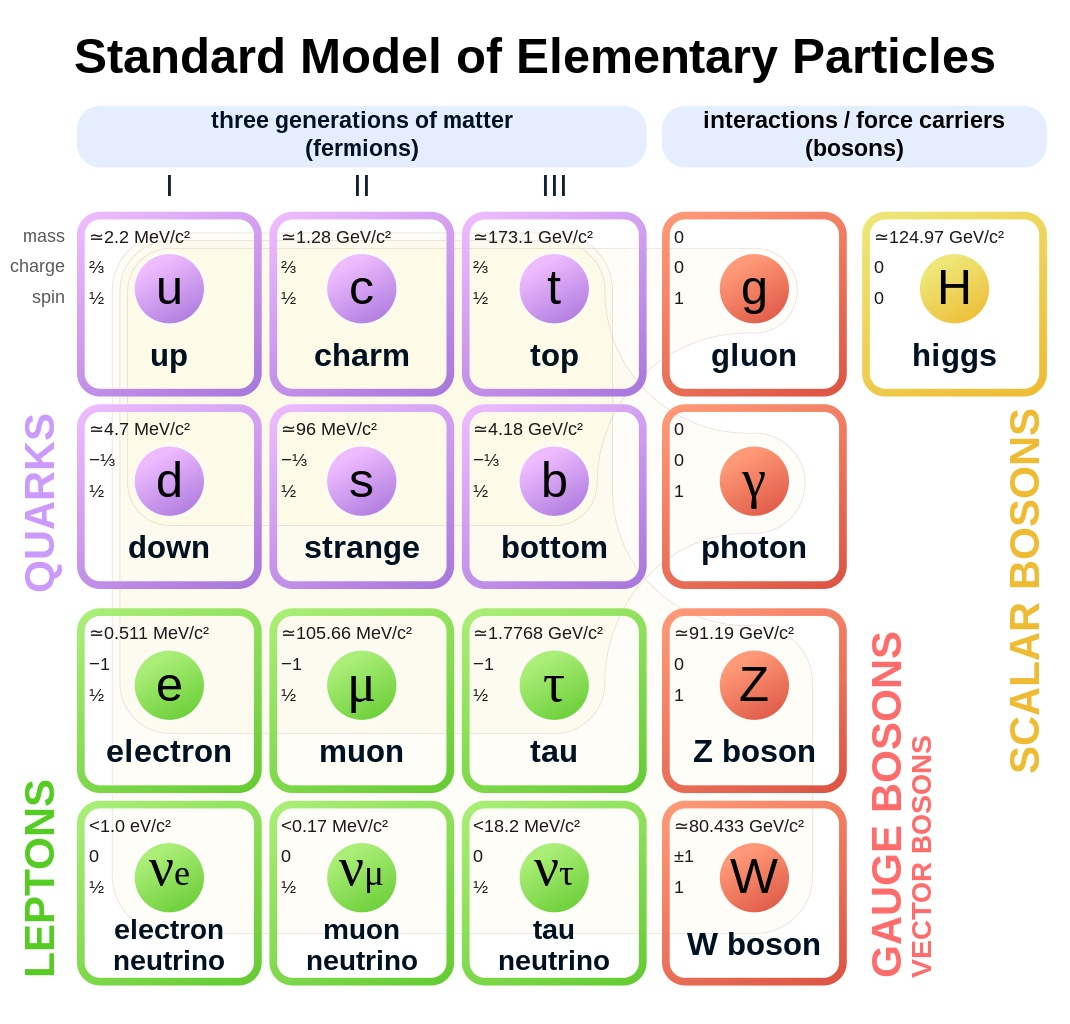
\includegraphics[width=0.6\linewidth]{/Users/samueljankovych/Documents/MFF/bakalarka/thesis/src/img/sm.jpg}
    \caption[The Standard Model of particle physics.]{The Standard Model of particle physics. \footnotemark}
    \label{fig:sm}
\end{figure}
\footnotetext{\url{https://en.wikipedia.org/wiki/File:Standard_Model_of_Elementary(P)articles.svg}}
\emph{Fermions} are particles that makeup all the matter and \emph{bosons} are force-mediating particles.
All known elementary particles are displayed in \cref{fig:sm}.

Fermions are split up into two categories, \emph{leptons} and \emph{quarks}. 
Leptons are further divided into two groups:
\begin{enumerate}
    \item  
    \begin{itemize}
        \item \emph{electron}, a particle that is present in all matter around us,
        \item \emph{muon}, a heavier cousin of electron naturally produced in the atmosphere,
        \item \emph{tau lepton}, the heaviest lepton.
    \end{itemize}
    These three leptons can interact via the \emph{Electromagnetic Force} (they have a charge), mediated by \emph{photons}, or via the \emph{Weak Force}, mediated by \emph{W and Z boson}. 
    \item \emph{Neutrinos}, each belonging to either electron, muon, or tau lepton.  
    Neutrinos can interact only weakly by exchanging W and Z bosons.
\end{enumerate}
Quarks are also divided into two groups:
\begin{multicols}{2}
\begin{enumerate}
    \item  
    With electric charge $\frac{2}{3}$ \footnote{Measured in units of elementary charge $e=1.60217663\cdot10^{-19}$ C.},
    \begin{itemize}
        \item \emph{up}, u quark,
        \item \emph{charm}, c quark,
        \item \emph{top}, t quark.
    \end{itemize}
    \item  
    With electric charge $-\frac{1}{3}$.
    \begin{itemize}
        \item \emph{down}, d quark,
        \item \emph{strange}, s quark,
        \item \emph{bottom}, b quark.
    \end{itemize}
\end{enumerate}
\end{multicols}
All quarks can interact not only weakly and electromagnetically, but also via the \emph{Strong Force}, mediated by \emph{gluons}.
In nature practically only the u-quark and d-quark occur, concretely they are the building blocks of protons and neutrons.

Fermions can be also split another way, into three families. 
The order of families is given by the mass of corresponding particles.
The lightest is built up by a u-quark, a d-quark, an electron, and an electron neutrino.
Practically all matter around us is made up of particles from this family.
It should be noted that neutrino masses are not exactly known.
Due to a measured process \cite{sadbury} called neutrino oscillations \cite{pdg}, they cannot be massless.
Since the first discovery, estimates on the upper bound of their masses were made \cite{pdg}.

The bosonic particles are a photon, gluon, W, and Z boson, and \emph{Higgs boson}. They can be split up into two groups:
\begin{enumerate}
    \item \emph{Vector Bosons}: photon, gluon, W and Z boson,
    \item \emph{Gauge Bosons}: Higgs boson.
\end{enumerate}
Vector bosons ('vector' comes from their mathematical description) are force carriers:
\begin{itemize}
    \item \emph{Electromagnetic Force} - photon,
    \item \emph{Strong Force} - gluon,
    \item \emph{Weak Force} - Z and W boson.
\end{itemize}
The nature of each force is given by the properties of the corresponding force-carrying boson.
The interaction strength of each force is given by the corresponding charge of interacting particles.

Particles that have electric charges can exchange photons and interact electromagnetically.
The infinite range of the Electromagnetic force is due to the photons being massless.
They also have no charge, which makes them unable to scatter on other photons.~\footnote{This has some caveats at higher energies. Classically it is forbidden due to the linearity of Maxwell's equations, but at higher orders of perturbation QFT, photons can scatter on another photon. However, the probability of such an event is very low.}

Gluons are also massless, making the Strong Force also infinite.
The only fermion carriers of the strong charge (also called \emph{color charge}) are quarks. 
Since gluons have two strong chargers, they can not only interact with other gluons but also exchange color charges when interacting with either quarks or gluons.
This is very different from Electromagnetic Interaction, where particles' charge does not change. 
Even though the Strong Interaction is theoretically infinite, due to a process called \emph{hadronization} (detailed description in ????), we do not see free gluons or quarks. 
They only occur in a bound state in nature, effectively making the color charge invisible at a larger scale (it becomes visible at~the~scale~of approximately 1 fm)

All fermions can interact weakly, but since W and Z bosons have mass (which is big compared to fermions), the range of interaction is short.
Naturally weak processes occur in $\beta$-decay.

Last, but not least is the Higgs boson, a scalar boson.
The strength of the interaction with the Higgs boson (more precisely: with the scalar field, Higgs field) is given by the mass of the interacting particle.
In other words, particles' interaction with the Higgs field gives them mass.
This makes gluons and photons the only particles from \SM non-interacting with the Higgs boson.



\section{Quantum Field Theory}
\label{sec:qft}
\QFT is a fundamental framework in modern theoretical physics that describes the behavior of particles and fields at the quantum level.
Its first development was done by studying the electromagnetic interaction of particles and photons by Paul Dirac \cite{dirac}.
Huge progress in \QED was made by Richard Feynman \cite{feynman}, who also introduced the \emph{Feynman diagrams}, a graphical representation of interactions.
We will discuss Feynman diagrams in more detail in \cref{sec:feyman}.

The starting point of QFT is the idea that particles are not fundamental objects but instead are excitations of underlying quantum fields that permeate all of space and time. 
This field must satisfy the equations of motion of the corresponding field theory, derived from the Lagrangian density of the theory.

\subsection{Free Particles}
\label{sec:free_particles}
The Lagrangian of non-interacting \spinhalf particle also called the \emph{Dirac Lagrangian}, is given by
\begin{equation}
    \label{eq:dirac_lag}
    \mathcal{L}_{\text{Dirac}} = \bar{\psi}(i\slashed{\partial} - m) \psi,
\end{equation}
where we abbreviate $\gamma^\mu \partial_\mu \equiv \slashed{\partial}$, $\gamma^\mu$ are the Dirac matrices, and $\partial_\mu$ is the covariant derivative.
$\psi(x)$ is a bispinor fermionic field of a spin $\frac{1}{2}$ particle. 
It has 4 components, which can be split into two spinors, each corresponding to a different chirality
\begin{equation}
    \psi(x) = \left( \begin{array}{c} \psi_L(x) \\ \psi_R(x) \end{array} \right).
\end{equation}
The Dirac equation is an equation of motion, derived from the Lagrangian \cref{eq:dirac_lag}:
\begin{equation}
    \label{eq:dirac_eq}
    \left( i \gamma^\mu \partial_\mu - m \right) \psi(x) = 0.
\end{equation}

Bosons on the other hand are spin-1 particles, described by the vector field $A_\mu(x)$.
The Lagrangian of a non-interacting spin-1 particle is given by a \emph{Proca Lagrangian}
\begin{equation}
    \label{eq:proca_lag}
    \mathcal{L}_{\text{Proca}} = - \frac{1}{4} F_{\mu\nu} F^{\mu\nu} + \frac{1}{2} m^2 A_\mu A^\mu,
\end{equation}
where $F_{\mu\nu} = \partial_\mu A_\nu - \partial_\nu A_\mu$ is the field strength tensor.
Note that this Lagrangian describes massive bosons, in the case of massless bosons, the second term is omitted.
The equation of motion for the vector field, Klein-Gordon equation:
\begin{equation}
    \label{eq:klein_gordon}
    \left( \Box - m^2 \right) A_\mu(x) = 0.
\end{equation}

\subsection{Interacting Particles}
\label{sec:interacting_particles}
We introduce the interaction between fields by invoking the \emph{local gauge invariance} of the Lagrangian. 
This means that the Lagrangian must be invariant under the transformation, which is a representation of an underlying \emph{Lie group}. 
Each interaction corresponds to a different type of a \emph{Lie group}.
For example, the electromagnetic interaction corresponds to U(1) group, which means that the Lagrangian must be invariant under the transformation
\begin{equation}
    \label{eq:gauge_inv_QED}
    \psi(x) = \eu^{-i e \omega(x)}\psi(x), \quad A_\mu'(x) = A_\mu(x) + \partial_\mu \omega(x),
\end{equation}
where $\omega(x)$ is a generator of the U(1) group.

In the general case of the non-Abelian SU(N) group having N different fermions with the free Lagrangian
\begin{equation}
    \label{eq:Dirac_N}
    \mathcal{L}_{\text{Dirac}} = \sum_{i=1}^N \bar{\psi}_i (i\slashed{\partial} - m) \psi_i,
\end{equation}
and $T^a$ ($a = 1,2,..., N$) being the generators of the SU($N$) group, the gauge transformation is given by
\begin{equation}
    \label{eq:gauge_inv}
    \psi_i(x)' = \sum_{j=1}^N \left( \eu^{-i g \alpha(x)^a T^a_{ij}}\right) \psi_j(x),
\end{equation}
where $\alpha(x)$ is the gauge field, and $g$ is the coupling constant.
We now have $N$ different bosonic fields, $A^a_\mu(x)$, each corresponding to a different generator $T^a$ (NxN matrices).
Their infinitesimal transformations are given by
\begin{equation}
    \label{eq:gauge_inv_bosons}
    A^a_\mu(x)' \rightarrow A^a_\mu(x) + \frac{1}{g} \partial_\mu \alpha^a(x) - f^{abc} \alpha^b(x) A^c_\mu(x),
\end{equation}
where $f^{abc}$ are the structure constants of the SU($N$) group
\begin{equation}
    \label{eq:structure_constants}
    [T^a, T^b] = i f^{abc} T^c.
\end{equation}
The field strength tensor is modified as 
\begin{equation}
    \label{eq:field_strength}
    F^a_{\mu\nu} = \partial_\mu A^a_\nu - \partial_\nu A^a_\mu + g f^{abc} A^b_\mu A^c_\nu.
\end{equation}
Finally, we obtain the interacting, SU(N) locally invariant,  Lagrangian
\begin{equation}
    \label{eq:lag_suN}
    \mathcal{L} = - \frac{1}{4}  F^a_{\mu\nu} F^a_{\mu\nu} + \frac{1}{2} m^2 A^a_\mu A^a_\mu, + \sum_{i,j=1}^N \bar{\psi}_i (i\delta_{ij} \slashed{\partial}  +g \slashed{A}^a T^a_{ij} - m \delta_{ij}) \psi_j.
\end{equation}


\subsection{Feynamn Diagrams}
\label{sec:feyman}









\section{Quantum Chromodynamics}
\label{sec:qed}

